\item The minimum eigenvalue of the following matrix is  
\hfill \brak{\text{EC 2013}}
\begin{align*}
    \myvec{ 3 & 5 & 2 \\ 5 & 12 & 7 \\ 2 & 7 & 5 }
\end{align*}
\begin{multicols}{4}
  \begin{enumerate}
\item 0
\item 1
\item 2
\item 3
\end{enumerate}
\end{multicols}
\item Let $\vec{A}$ be an $m \times n$ matrix and $\vec{B}$ an $n \times m$ matrix. It is given that $\det\brak{\vec{I}_m + \vec{A}\vec{B}} = \det\brak{\vec{I}_m + \vec{A}\vec{B}}$. Using this property, the determinant of the matrix
$\myvec{2 & 1 & 1 & 1 \\
1 & 2 & 1 & 1 \\
1 & 1 & 2 & 1 \\
1 & 1 & 1 & 2}$
is

\hfill \brak{\text{EC 2013}}
\begin{multicols}{4}
\begin{enumerate}
\item 2
\item 5
\item 8
\item 16
\end{enumerate}
\end{multicols}
\item The DFT of a vector \myvec{a&b&c&d} is the vector \myvec{\alpha&\beta&\gamma&\delta}. Consider the product
$$\myvec{p&q&r&s} = \myvec{a&b&c&d} 
\myvec{
a & b & c & d \\
d & a & b & c \\
c & d & a & b \\
b & c & d & a}.$$
The DFT of the vector \myvec{p&q&r&s} is a scaled version of
\hfill \brak{\text{EC 2013}}
\begin{multicols}{2}
\begin{enumerate}
\item $\myvec{\alpha^2&\beta^2&\gamma^2&\delta^2}$
\item $\myvec{\alpha+ \beta&\beta+\delta &\delta+\gamma&\gamma + \alpha}$
\item $\myvec{\sqrt{\alpha}&\sqrt{\beta}&\sqrt{\gamma}&\sqrt{\delta}}$
\item $\myvec{\alpha&\beta&\gamma&\delta}$
\end{enumerate}
\end{multicols}
\item The state diagram of a system is shown below in \figref{fig:placeholder_23}. A system is described by the state-variable equations
\begin{align*}
    \dot{\vec{X}} = \vec{A}\vec{X} + \vec{B}\vec{u}; \ \ \ \ y= \vec{C}\vec{X}+\vec{D}\vec{u}
\end{align*}
\begin{figure}[H]
    \centering
    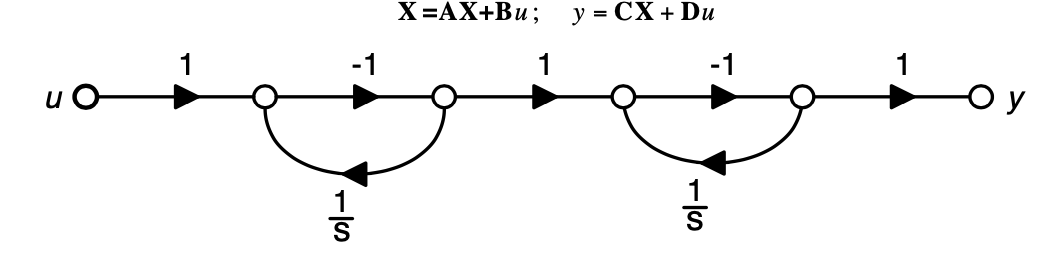
\includegraphics[width=0.5\columnwidth]{GATE/2013/EC/figs/fig_23.png}
    \caption{}
    \label{fig:placeholder_23}
\end{figure}
The state-variable equations of the system shown in the figure above are
\hfill \brak{\text{EC 2013}}
\begin{multicols}{2}
\begin{enumerate}
	\item \begin{align*}\dot{\vec{X}}&= \myvec{-1&&0\\1&&-1} \vec{X} + \myvec{-1 \\ 1} \vec{u} \\ \vec{y}&=\myvec{1 && -1}\vec{X} + \vec{u}\end{align*}
    \item \begin{align*}\dot{\vec{X}}&= \myvec{-1&&0\\-1&&-1} \vec{X} + \myvec{-1 \\ 1} \vec{u} \\ \vec{y}&=\myvec{-1 && -1}\vec{X} + \vec{u}\end{align*}  
    \item \begin{align*}\dot{\vec{X}}&= \myvec{-1&&0\\-1&&-1} \vec{X} + \myvec{-1 \\ 1} \vec{u} \\ \vec{y}&=\myvec{-1 && -1}\vec{X} - \vec{u}\end{align*}
    \item \begin{align*}\dot{\vec{X}}&= \myvec{-1&&-1\\0&&-1} \vec{X} + \myvec{-1 \\ 1} \vec{u} \\ \vec{y}&=\myvec{1 && -1}\vec{X} - \vec{u}\end{align*}
\end{enumerate}
\end{multicols}

